\newpage
\section{Appendix: Algorithms for Sampling and Inference}
\label{app:algorithms}

In this section, we provide the detailed algorithms for sampling and inference using our Structured Flow Matching framework. We distinguish between two conditioning paradigms: \texttt{Static} (for sequential sampling) and \texttt{Dynamic} (for parallel sampling); Figure~\ref{fig:static-v-dynamic-conditioning} contrasts the two schematically.

\begin{figure}[H]
    \centering
    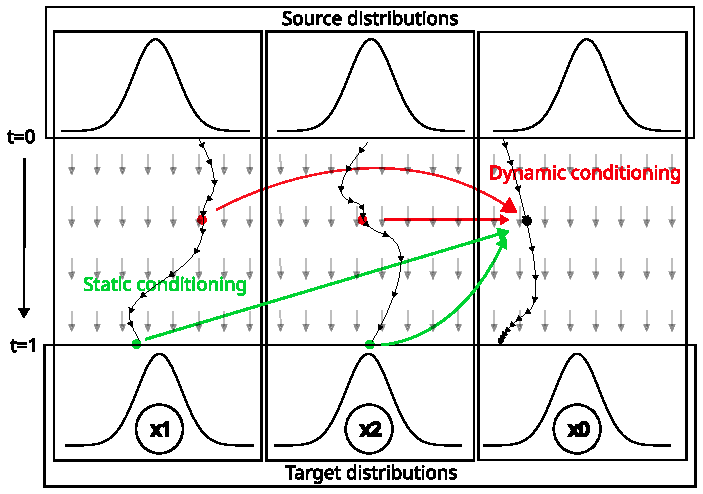
\includegraphics[width=0.72\textwidth]{images/collider-pgm-structured.pdf}
    \caption{\textbf{Static vs.\ Dynamic Conditioning.} Sampling $p(x_0 \mid x_1, x_2)$ with a block-triangular flow ordered $[x_1, x_2, x_0]$ (e.g.\ compiled from the collider $X_1 \to X_0 \leftarrow X_2$). Static conditioning (green) first integrates the conditioning blocks to completion and provides their final values $x_1^{(t=1)}, x_2^{(t=1)}$ as fixed inputs to the velocity field of $x_0$. Dynamic conditioning (red) integrates all blocks jointly in a single ODE solve, with $x_0$'s velocity conditioned on the evolving trajectories $x_1^{(t)}, x_2^{(t)}$ at each time step.}
    \label{fig:static-v-dynamic-conditioning}
\end{figure}

\subsection{Static Conditioning}

\subsubsection{Static Sampling}

In the Static mode, variables are sampled sequentially following a topological ordering of the dependency graph. Each variable's flow is conditioned on the \textit{final} values ($t=1$) of its parents. This minimizes the number of variables in any single ODE solve but requires $K$ separate integration passes for $K$ target variables.

\begin{algorithm}[H]
\caption{Static Conditional Sampling}
\label{alg:static_sampling}
\begin{algorithmic}
\REQUIRE Trained Velocity Field $v_\phi$, Observations $c$, Target variables $\Theta$
\ENSURE Samples $\theta_{t=1}$
\STATE $Order \gets \text{TopoSort}(\Theta \text{ with respect to } \text{Parents}(\Theta))$
\STATE $Context \gets c$ (Initial static conditions)
\FOR{$y \in Order$}
    \STATE Sample noise $z_y \sim \mathcal{N}(0, I)$
    \STATE Define single-block ODE: $\frac{dy}{dt} = v_\phi^{(y)}(t, y, Context)$
    \STATE Integrate $t: 0 \to 1$ starting from $y(0) = z_y$
    \STATE $Context[y] \gets y(1)$ (Update context for downstream blocks)
    \ENDFOR
    \STATE \textbf{return} $Context[\Theta]$
    \end{algorithmic}
\end{algorithm}

\subsubsection{Static Density Evaluation}

For static conditioning, the conditional log-probability $\log p(y_{targets} | y_{conditions})$ is computed by integrating the flow ODE backward from $t=1$ to $t=0$. By Proposition~\ref{prop:cond-density}, we compute the log-density by accumulating the divergence of the target variables only. Because the flow has a block-triangular Jacobian, the log-determinant term decomposes into a sum over individual blocks, allowing us to ignore the divergence of the conditioning variables.

\subsection{Dynamic Conditioning}

\subsubsection{Dynamic Sampling}

In the Dynamic mode, all variables are integrated simultaneously in a single monolithic ODE solve. This requires reproducing the full temporal trajectories ($t \in [0, 1]$) of the conditioning variables. While this approach requires a more complex trajectory-interpolation step, it allows the sampling process to be parallelized across blocks, which is advantageous for deep or highly connected graphs.

\begin{algorithm}[H]
\caption{Dynamic Conditional Sampling}
\label{alg:dynamic_sampling}
\begin{algorithmic}
\REQUIRE Trained Velocity Field $v_\phi$, Observations $c$, Target variables $\Theta$
\ENSURE Samples $\theta_{pred}$
\STATE $\mathcal{B} \gets \text{AllBlocks}()$ (All variable blocks in the model)
\STATE $\mathcal{C} \gets \text{Keys}(c)$ (Condition blocks from observations)
\STATE $\mathcal{S} \gets \text{RequiredSimulationBlocks}(\Theta, \mathcal{C})$ (Ancestors of $\Theta$ not in $\mathcal{C}$)
\STATE $z_{dict} \gets \{\}$
\IF{conditions $c$ provided}
    \STATE Construct $x^{(1)}_{cond}$ with observed values $c[\mathcal{C}]$ and zeros elsewhere
    \STATE Integrate backward $t: 1 \to 0$: $\frac{dx}{dt} = v_\phi(t, x)$ from $x(1) = x^{(1)}_{cond}$
    \STATE Extract $z_{cond} \gets z(0)$ for condition blocks only
    \STATE $z_{dict} \gets z_{cond}$
\ENDIF
\STATE $\text{ToSample} \gets \{b \in \mathcal{S} : b \notin z_{dict}\}$ (Blocks needing fresh noise samples)
\FOR{$b \in \text{ToSample}$}
    \STATE Sample $z_b \sim \mathcal{N}(0, I)$
    \STATE $z_{dict}[b] \gets z_b$
\ENDFOR
\STATE Fill remaining blocks: For $b \in \mathcal{B} \setminus z_{dict}$, sample or set to zero
\STATE Construct $x^{(0)} \gets \text{Flatten}(z_{dict})$ (Concatenate all noise blocks in order)
\STATE Integrate forward $t: 0 \to 1$: $\frac{dx}{dt} = v_\phi(t, x)$ from $x(0) = x^{(0)}$
\STATE $x^{(1)} \gets x(1)$
\STATE \textbf{return} $\text{Unflatten}(x^{(1)})[\Theta]$ (Extract target variables)
\end{algorithmic}
\end{algorithm}

The zero padding is allowed as parents are not dependent on children, and the conditions are guaranteed to be parents. Therefore, the zero padding has no effect on the backward simulation of the conditions.

\subsubsection{Dynamic Density Evaluation}

In the Dynamic (parallel) mode, density evaluation requires reconstructing the full temporal trajectories of the conditioning variables. We first integrate the full system (targets + conditions) backward from $t=1$ to $t=0$ to obtain the trajectories $\tau_{all}(t)$. We then define a subset velocity field $v_T(y_T, t; \tau_C)$ where the conditioning variables are interpolated from their backward trajectories. By Proposition~\ref{prop:cond-density}, we compute the log-density by accumulating the divergence of the target variables only, properly accounting for the dynamic coupling between variables without integrating the full joint density.